The authentication protocol is illustrated in \autoref{fig:password_protocol}.
\begin{figure}
    \centering
    \tikzset{every picture/.style={line width=0.75pt}} %set default line width to 0.75pt        

    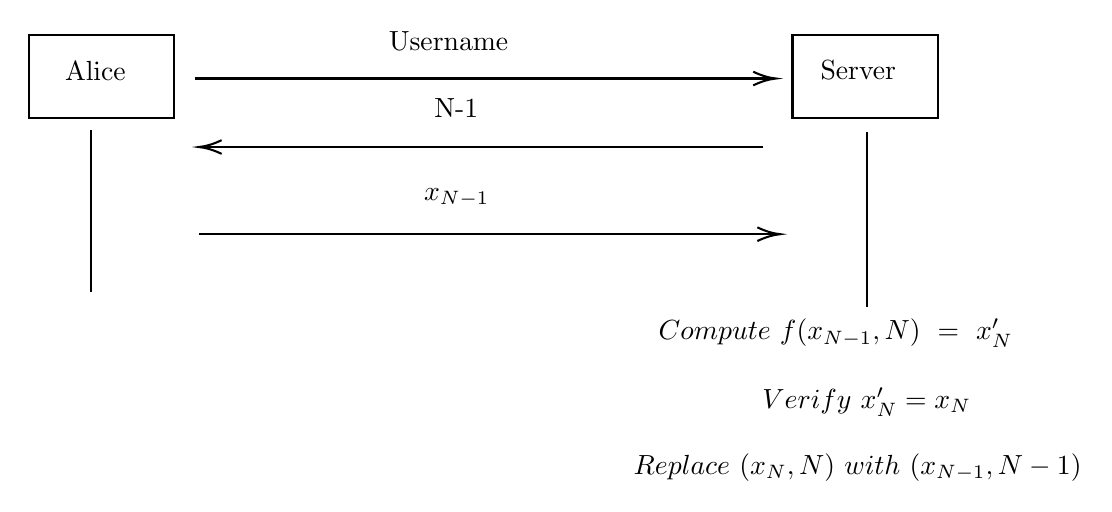
\begin{tikzpicture}[x=0.75pt,y=0.75pt,yscale=-1,xscale=1]
    %uncomment if require: \path (0,300); %set diagram left start at 0, and has height of 300

    %Shape: Rectangle [id:dp9302056250655825] 
    \draw   (108,32) -- (178,32) -- (178,72) -- (108,72) -- cycle ;

    %Shape: Rectangle [id:dp8316101362016359] 
    \draw   (476,32) -- (546,32) -- (546,72) -- (476,72) -- cycle ;

    %Straight Lines [id:da8540576995480886] 
    \draw    (188,53) -- (466,53) ;
    \draw [shift={(468,53)}, rotate = 180] [color={rgb, 255:red, 0; green, 0; blue, 0 }  ][line width=0.75]    (10.93,-3.29) .. controls (6.95,-1.4) and (3.31,-0.3) .. (0,0) .. controls (3.31,0.3) and (6.95,1.4) .. (10.93,3.29)   ;
    %Straight Lines [id:da9236128666658007] 
    \draw    (138,78) -- (138,156) ;
    %Straight Lines [id:da4298900090363067] 
    \draw    (512,79) -- (512,163) ;
    %Straight Lines [id:da6626236203364586] 
    \draw    (462,86) -- (192,86) ;
    \draw [shift={(190,86)}, rotate = 360] [color={rgb, 255:red, 0; green, 0; blue, 0 }  ][line width=0.75]    (10.93,-3.29) .. controls (6.95,-1.4) and (3.31,-0.3) .. (0,0) .. controls (3.31,0.3) and (6.95,1.4) .. (10.93,3.29)   ;
    %Straight Lines [id:da41522984839829913] 
    \draw    (190,128) -- (468,128) ;
    \draw [shift={(470,128)}, rotate = 180] [color={rgb, 255:red, 0; green, 0; blue, 0 }  ][line width=0.75]    (10.93,-3.29) .. controls (6.95,-1.4) and (3.31,-0.3) .. (0,0) .. controls (3.31,0.3) and (6.95,1.4) .. (10.93,3.29)   ;

    % Text Node
    \draw (124,43) node [anchor=north west][inner sep=0.75pt]   [align=left] {Alice};
    % Text Node
    \draw (488,43) node [anchor=north west][inner sep=0.75pt]   [align=left] {Server};
    % Text Node
    \draw (280,29) node [anchor=north west][inner sep=0.75pt]   [align=left] {Username};
    % Text Node
    \draw (302,61) node [anchor=north west][inner sep=0.75pt]   [align=left] {N-1};
    % Text Node
    \draw (297,104.4) node [anchor=north west][inner sep=0.75pt]    {$x_{N-1}$};
    % Text Node
    \draw (410,167.4) node [anchor=north west][inner sep=0.75pt]    {$Compute\ f( x_{N-1} ,N) \ =\ x'_{N}$};
    % Text Node
    \draw (460,200.4) node [anchor=north west][inner sep=0.75pt]    {$Verify\ x'_{N} =x_{N}$};
    % Text Node
    \draw (398,232.4) node [anchor=north west][inner sep=0.75pt]    {$Replace\ ( x_{N} ,N) \ with\ ( x_{N-1} ,N-1)$};

    \end{tikzpicture}

    \caption{Authentication protocol.(Exercise 8)}\label{fig:password_protocol}

\end{figure}

\subsection*{a) Advantages over using ordinary passwords}
%

\begin{itemize}
    \item Easy to detect if an attacker unauthorizedly use your password
    to access the server: Since the server would replace the values
    \((x_N,N)\) with the values \(x_(N-1),N-1\) after each successful
    user authentication, when the server request for the value \emph{N-1}
    which you don't have, that's a moment you realize that someone did
    attack your password (in this case the attacker just passively explore
    what can do with your account without changing your password).
    \item If the database storing \((x_i,i)\) is compromised, these leaked
    information are able to be used once since the entry \((x_i,i)\) changes
    every successful authentication. However, if the user log-in at least
    one more time after the pair \((x_i,i)\) is leaked, then the compromised
    pair is invalid.
\end{itemize}

\subsection*{b) Possible attacks}
%
\begin{itemize}
    \item The pair \((x_i,i)\) is easily captured by the attacker as it is not
    encrypted.
    \item The attacker can impersonate the server and re-send \(N-1,\cdots,1\)
    to Alice to retrieve \(x_N,\cdots,x_1\).
\end{itemize}